\documentclass[12pt]{article}
\usepackage[margin=1in]{geometry} 
\usepackage[normalem]{ulem}
\usepackage{graphicx,amssymb,multirow,amsmath,amsthm,psfrag,setspace,subfigure,float,cite,authblk,color,url,mathtools,indentfirst}
\usepackage{xeCJK}
\usepackage{amsxtra}
\usepackage{amsthm,amsmath,amssymb}
\usepackage{mathrsfs}
\usepackage[colorlinks=true,bookmarks=true]{hyperref}
%\usepackage{breakurl} %%This package must be after hyperref
\usepackage{float}
\usepackage{cite}
\usepackage{graphicx} 
\usepackage{listings}
\lstset{breaklines}  %让LaTeX自动将长的代码行换行排版
\usepackage{color}
\usepackage{appendix}
\usepackage{caption}
\definecolor{dkgreen}{rgb}{0,0.6,0}
\definecolor{gray}{rgb}{0.5,0.5,0.5}
\definecolor{mauve}{rgb}{0.58,0,0.82}
\usepackage[table,xcdraw]{xcolor}
\usepackage{authblk}
\usepackage{siunitx}
\lstset{
  language=C,                % the language of the code
  basicstyle=\footnotesize,           % the size of the fonts that are used for the code
  numbers=left,                   % where to put the line-numbers
  numberstyle=\tiny\color{gray},  % the style that is used for the line-numbers
  stepnumber=1,                   % the step between two line-numbers. If it's 1, each line 
                                  % will be numbered
  numbersep=5pt,                  % how far the line-numbers are from the code
  backgroundcolor=\color{white},      % choose the background color. You must add \usepackage{color}
  showspaces=false,               % show spaces adding particular underscores
  showstringspaces=false,         % underline spaces within strings
  showtabs=false,                 % show tabs within strings adding particular underscores
  frame=single,                   % adds a frame around the code
  rulecolor=\color{black},        % if not set, the frame-color may be changed on line-breaks within not-black text (e.g. commens (green here))
  tabsize=2,                      % sets default tabsize to 2 spaces
  captionpos=b,                   % sets the caption-position to bottom
  breaklines=true,                % sets automatic line breaking
  breakatwhitespace=false,        % sets if automatic breaks should only happen at whitespace
  title=\lstname,                   % show the filename of files included with \lstinputlisting;
                                  % also try caption instead of title
  keywordstyle=\color{blue},          % keyword style
  commentstyle=\color{dkgreen},       % comment style
  stringstyle=\color{mauve},         % string literal style
  escapeinside={\%*}{*)},            % if you want to add LaTeX within your code
  morekeywords={*,...}               % if you want to add more keywords to the set
}
\graphicspath{{fig/}}


\numberwithin{equation}{section}


\newcommand{\mbr}{\mathbb{R}}
\title{Project Report: Temperature Controlled LED Circuit}
\author[*]{Guo Yiming}
\affil[*]{
    Department of Physics, Xiamen University Malaysia}
\renewcommand\Authands{ and }


\begin{document}
\maketitle


\abstract{This report describes a circuit according to the temperature controlled LED. People can realize the temperature warning by adjusting the threshold temperature. This report also gives a variety of derivative circuits.}


\section{Introduction}

In real life, there are often some environments or equipment that require the upper limit of temperature. For example, for libraries or archives, too high temperature may lead to the destruction of documents, for kitchens, appropriate temperature can improve the quality of cooking, or just for individuals, too high room temperature may lead to heatstroke and other problems. Therefore, I designed an automatic temperature control LED warning light, which allows users to adjust the required temperature from \qtyrange{2}{100}{\degreeCelsius}. When the temperature exceeds the specified value, the LED will change from green to red to indicate a warning This equipment can help people to be more alert to temperature.

\section{Analysis}
\subsection{Main Component in Circuit}
Here first introduce several components and their special feature, which will be important to later analysis.


\subsubsection{LM35 Temperature Sensor\cite{LM35}}

\verb|LM35| has three pins,named as \verb|VS|, \verb|VOUT|, \verb|GND|, here in the circuit we are applying 	\textbf{Basic Contigrade Temperature Sensor} \cite{LM35} ,as below graph [\ref{Fig.basic_contigrade}]:

\begin{figure}[H] %H为当前位置,!htb为忽略美学标准,htbp为浮动图形
\centering %图片居中

\includegraphics[width=0.3\textwidth]{LM35_basic_centigrade} %插入图片,[]中设置图片大小,{}中是图片文件名
\caption{Basic Contigrade Temperature Sensor} %最终文档中希望显示的图片标题
\label{Fig.basic_contigrade} %用于文内引用的标签
\end{figure}


\verb|VS| is connected to the \verb|VS| which required to be \qtyrange{4}{20}{V}, \verb|GND| is connected on the ground. The output,\verb|VOUT| outputs a voltage proportional to temperature, and its relationship is as follows [\ref{equation.LM35}]\cite{LM35}:
\begin{equation}
	V_{out}=T \cdot \qty{10}{mV \per \degreeCelsius}  \label{equation.LM35}
\end{equation}

Where the temperature is in degrees Celsius In this wiring mode, the measured temperature is limited at \qtyrange{2}{100}{\degreeCelsius},


\subsubsection{LM358AD Operational Amplifier \cite{LM358AD}}
In the circuit, \verb|LM358AD| is used as a comparator to compare the two input voltages. When the \verb|+| port is large, \verb|VOUT| outputs high level voltage, which is the $V_ {CC} - \num{1.5}$ in this circuit, it is about \qty{3.5}{V}(ignoring the change caused by temperature)\cite{LM358AD}. When the \verb|-| port is large, \verb|VOUT| outputs low level voltage, which approximately could be regard as \qty{0}{V}. This Op-Amp acts as a switch in the circuit to respond to \verb|LM35| temperature change and convert it into instantaneous voltage jump, which will be used in later analysis.Here make a test on the \verb|LM358AD| with the function of camparator($\verb|V2|=\qty{2}{V}$,Apply \verb|DC sweep| on \verb|V1| from \qtyrange{0}{5}{V},increment as $0.1$,output \verb|VOUT|):


\begin{figure}[H]
\centering
\begin{minipage}[t]{0.48\textwidth}
\centering
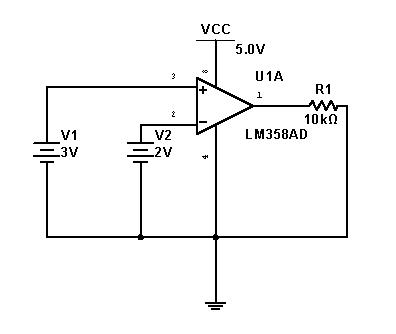
\includegraphics[height=5cm]{LM358_test.pdf}
\caption{LM358AD test circuit}
\label{fig.LM35}
\end{minipage}
\begin{minipage}[t]{0.48\textwidth}
\centering
\includegraphics[height=5cm]{LM358AD_test.eps}
\caption{$V_{OUT}$ voltage diagram}
\end{minipage}
\end{figure}












\subsubsection{BC547A NPN-type Transistor \cite{BC547A}}
\verb|BC547A| is a NPN-type transistor, it works as the direct switch for the LED light through controlling $V_{BE}$. By refering the datasheet\cite{BC547A}.The saturation voltage of $V_{BE} \approx \qty{0.7}{V}$.The \verb|BC| connected when $V_{BE} >0.7$, otherwise, it is open circuit.

\begin{figure}[H]
\centering
\begin{minipage}[t]{0.48\textwidth}
\centering
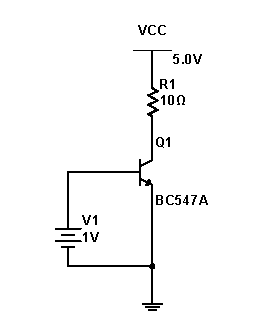
\includegraphics[height=5cm]{BC547A_test.pdf}
\caption{BC547A test circuit}
\label{fig.BC547A}
\end{minipage}
\begin{minipage}[t]{0.48\textwidth}
\centering
\includegraphics[height=5cm]{BC547A_test.eps}
\caption{$I_{R1}$ voltage diagram}
\end{minipage}
\end{figure}


\subsubsection{LED light}
Here in this report include three kinds of LED light which are red,green and blue, the turn on voltage is \qty{1.83}{V},\qty{2.13}{V} and \qty{3.45}{V} respectively.All their turn on current at \qty{20}{mA}.In furthere analysis we use the \textbf{Simplified Equivalent Circuit} model to analysis the LED circuit.



%TODO 这里引用后面的模块里的等效电路
\subsection{Module Analysis}


Next we apply analysis the whole circuit module by module seperately[\ref{Fig.module}].


\begin{figure}[H] %H为当前位置,!htb为忽略美学标准,htbp为浮动图形
\centering %图片居中
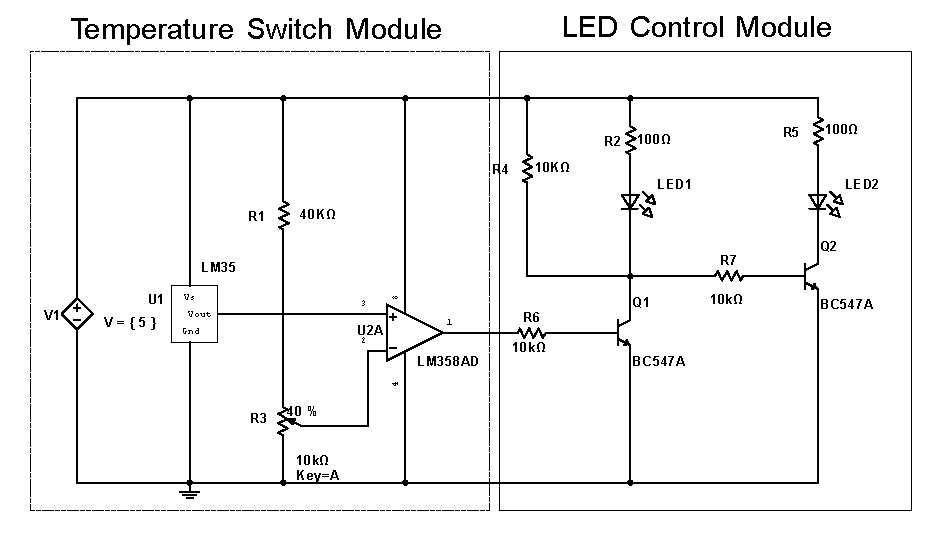
\includegraphics[width=0.8\textwidth]{module} %插入图片,[]中设置图片大小,{}中是图片文件名
\caption{Circuit Devided into Module} %最终文档中希望显示的图片标题
\label{Fig.module} %用于文内引用的标签
\end{figure}








\subsubsection{Temperature Switch Module}

This part is constructed \verb|LM358A| Op-Amp, \qty{10}{K\ohm} potentiometer, and a \qty{40}{K\ohm} resistor, connected as below circuit [\ref{Fig.temp_switch_sensor}]. 
The percentage,$p$, shown in the circuit diagram [\ref{Fig.temp_switch_sensor}] refers to the proportion of the upper part of the pointer, which follow the equation below:


\begin{figure}[H] %H为当前位置,!htb为忽略美学标准,htbp为浮动图形
\centering %图片居中
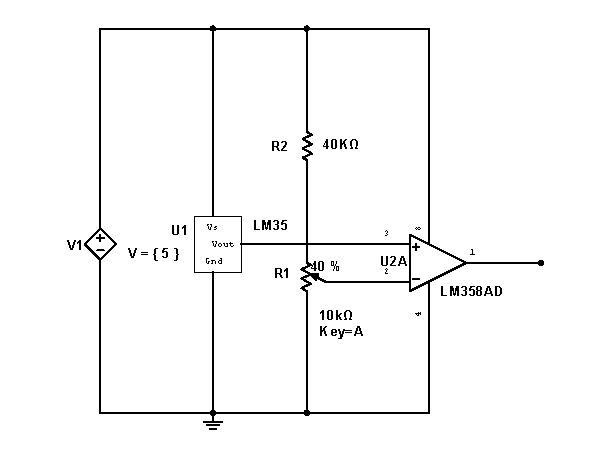
\includegraphics[width=0.8\textwidth]{Temperature_Switch_module_origin} %插入图片,[]中设置图片大小,{}中是图片文件名
\caption{Temperature Switch Module} %最终文档中希望显示的图片标题
\label{Fig.temp_switch_sensor} %用于文内引用的标签
\end{figure}



\begin{equation}
	V_-=\frac{(1-p) \cdot \qty{10}{K \ohm}}{\qty{40}{K \ohm}+\qty{10}{K \ohm}} \cdot \qty{5}{V}=(1-p)\unit{V}
\end{equation}

 
High resistance is used here to reduce the influence between other parts of the circuit and maintain the stability of the circuit.

For \verb|LM358AD|, when $V + > V_-$, $V_{out} $ will output $V_{CC} - \qty{1.5}{V}=3.5V $, and when $V_- > V_+$, $V_ {out}$ will output $0$.By the introduction in [\ref{equation.LM35}].Therefore we can conclude the result of the threshold temperature for \verb|LM358AD| to switch its output state:

\begin{equation}
	T_{\text{Thresold}}=100 \cdot p \unit{K}
\end{equation} 



After understanding the functional relationship between the voltage on the two pin ports and related factors, we can simply test this module. First, we adjust the potentiometer to $40\%$, that is, set the threshold temperature to \qty{60}{\degreeCelsius}. We perform temperature sweep on the circuit, set the start temperature to 0, set the cut-off temperature to \qty{100}{\degreeCelsius}, and set \num{100} sampling points, The sampling interval is about 1.01c, making it output \verb|V+|,\verb|V-|,\verb|VOUT| is the result, and the following chart is obtained [\ref{Fig.temp_switch_diagram}]:
% TODO 插入模块图像,图标图像 
%TODO 这里哈休要标注一下各个net的编码.

\begin{figure}[H] %H为当前位置,!htb为忽略美学标准,htbp为浮动图形
\centering %图片居中
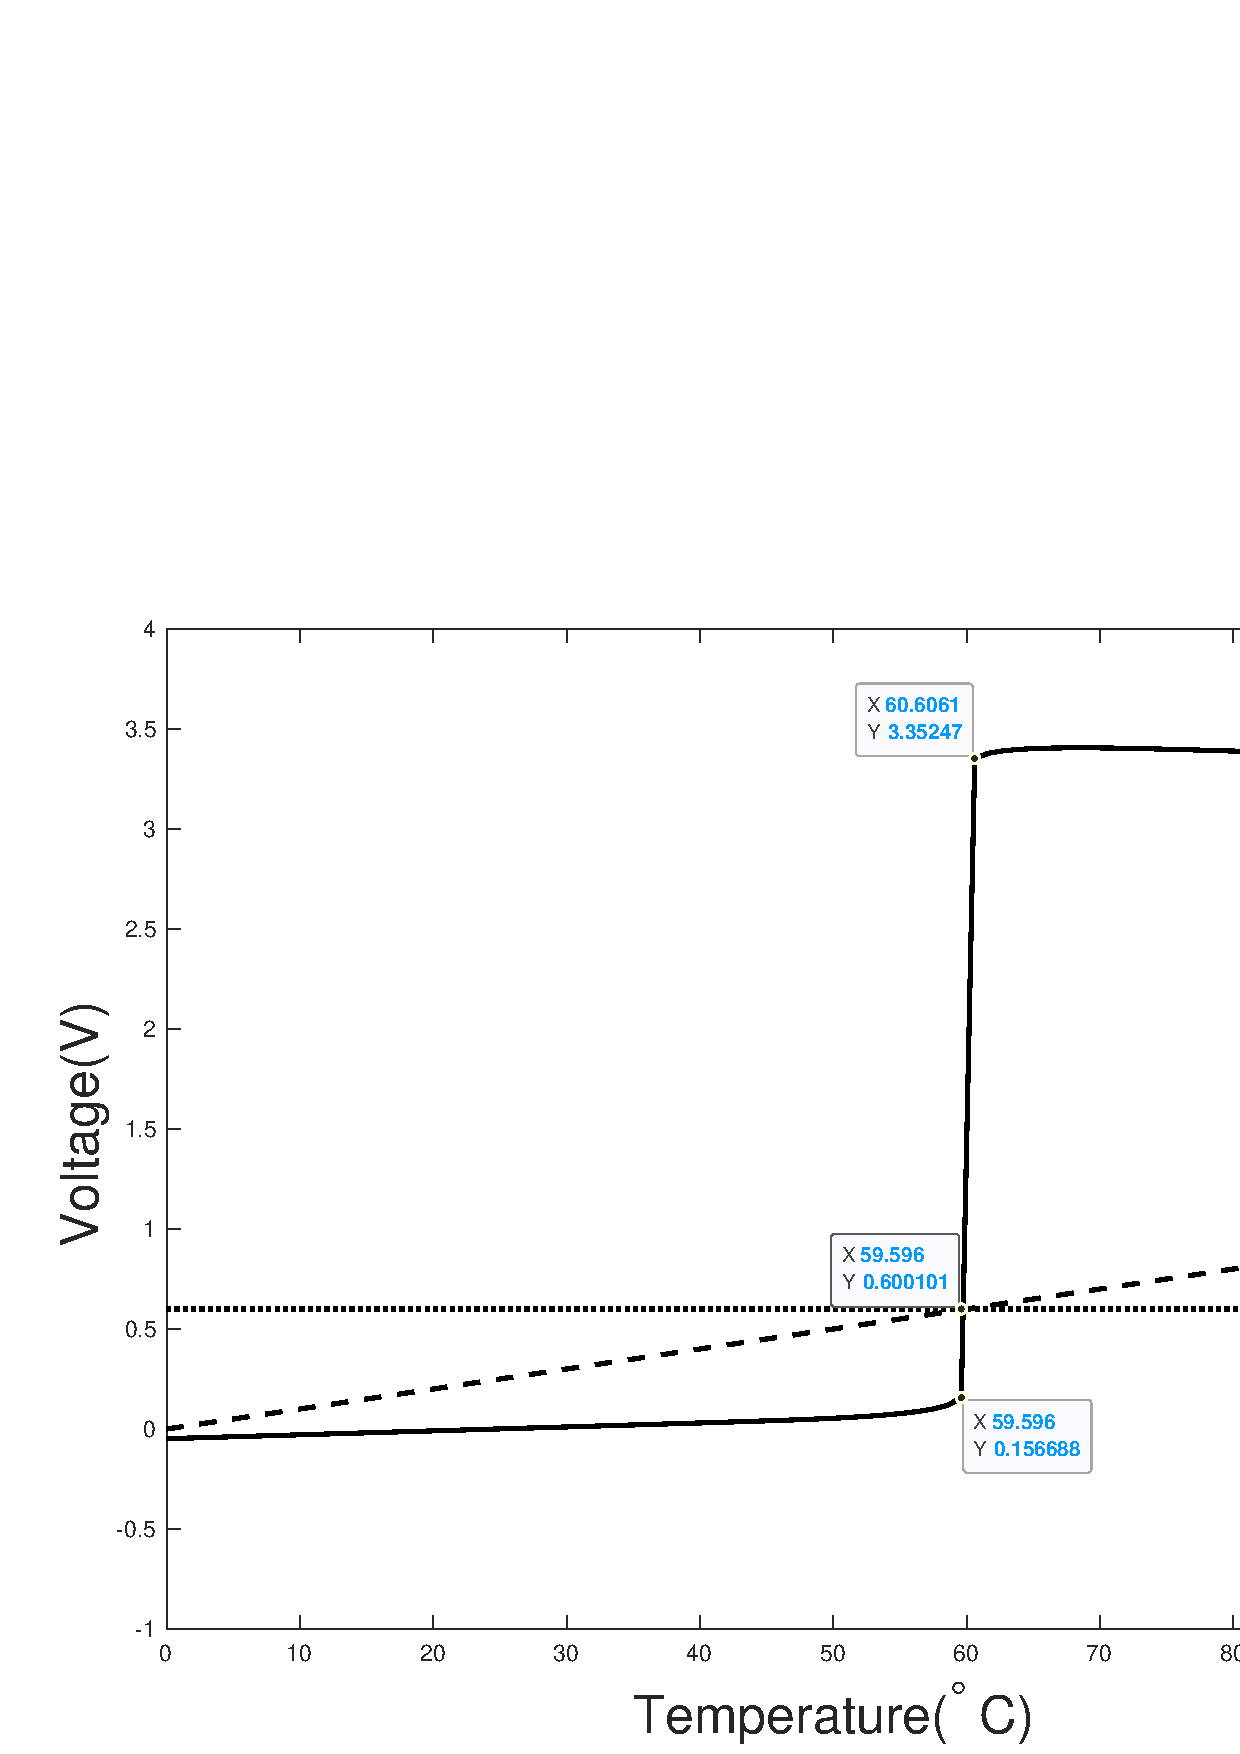
\includegraphics[width=0.8\textwidth]{temperature_switch_diagram} %插入图片,[]中设置图片大小,{}中是图片文件名
\caption{Temperature Switch Diagram Voltage($V+$,$V-$,$V_{OUT}$)} %最终文档中希望显示的图片标题
\label{Fig.temp_switch_diagram} %用于文内引用的标签
\end{figure}





It can be seen that the voltage at the \verb|V+| port increases linearly with the temperature. When the temperature reaches \qty{100}{\degreeCelsius}, the voltage is qty{1}{V}. At the same time, since we adjust the potentiometer at at $40\%$, the voltage of \verb|V-| is always constant at \qty{0.6}{V}. Therefore, we can see that \verb|V+| and \verb|V-| cross \qty{60}{\degreeCelsius}, which is \verb|VOUT| jumps from low level to high level.

%TODO 插入模块图像,图标图像
This is the working principle of the temperature switch module.



\subsubsection{LED Control Module}


For LED control module[\ref{Fig.LED_module}], we use two NPN-type BJT \verb|BC547a| as control switches, labelled as \verb|Q1| and \verb|Q2|. Two LED lights are connected in series with two \qty{100}{\ohm} resistors, \verb|R2| and \verb|R5| to control the current and prevent the LED lights from burning. Due to excessive current \verb|R5| is a large resistance of \qty{10}{K\ohm}, which is used to reduce the current through the the \verb|B| port of \verb|Q2| and keep the voltage between the \verb|VOUT| and the \verb|B| port of \verb|Q2|. \verb|R7| is a large resistance of \qty{10}{K\ohm}, which is used to reduce $I_B$ of \verb|Q2|, while maintaining voltage of \verb|C| port of \verb|Q1| and \verb|B| port of \verb|Q2| consistent, and \verb|R4| is used to protect the circuit and keep the circuit stable.


\begin{figure}[H] %H为当前位置,!htb为忽略美学标准,htbp为浮动图形
\centering %图片居中
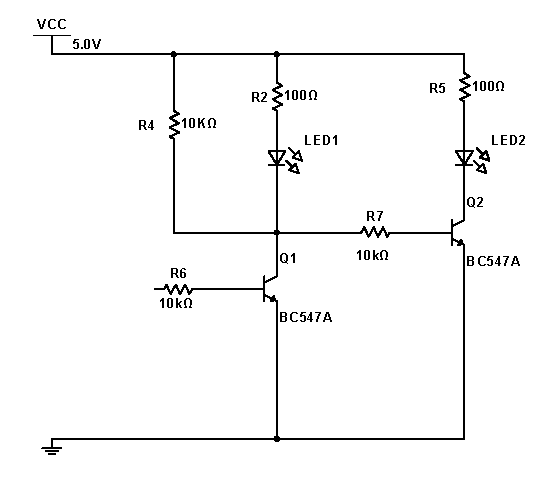
\includegraphics[width=0.8\textwidth]{LED_module} %插入图片,[]中设置图片大小,{}中是图片文件名
\caption{LED Module} %最终文档中希望显示的图片标题
\label{Fig.LED_module} %用于文内引用的标签
\end{figure}



Then start to analyze the circuit operation mode. First, the output from Op-Amp can only be high level(\qty{3.5}{V}) or low level(\qty{0}{V}). Therefore, we first assume that the left end through \verb|R6| is high level, and then $I_{R6}$ is almost \num{0}, $V_{D} \approx V_ {C}= V_{\text{Oh}} \approx \qty{3.5}{V}$, so the \verb|CE| port of \verb|Q1| are connected (here we assume that BJT is ideal), and $V_E=V_{GND}=0 $. Due to $I_{R_6} \approx I_{R_4} \approx 0 $, so $V_{BE} \approx 0$, the \verb|CE| of \verb|Q2| is not conductive, so the equivalent circuit can be drawn. It is easy to see that only \verb|LED1| is conductive at this time. At the same time, considering that the LED is a red LED, the circuit can be simplified as:



\begin{figure}[H]
\centering
\begin{minipage}[t]{0.48\textwidth}
\centering
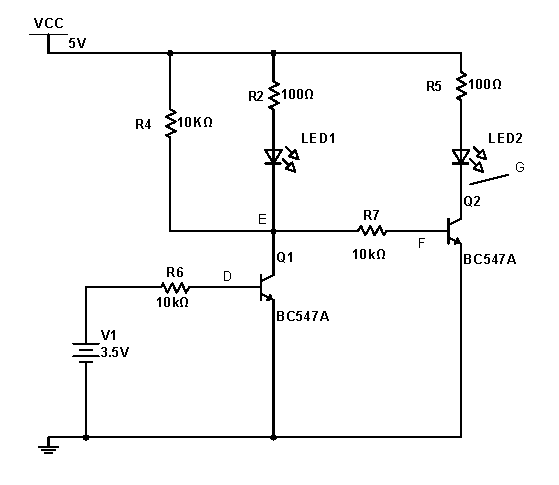
\includegraphics[height=6cm]{LED_module_hi_1.pdf}

\caption{$V_D=3.5V$}
\end{minipage}
\begin{minipage}[t]{0.48\textwidth}
\centering
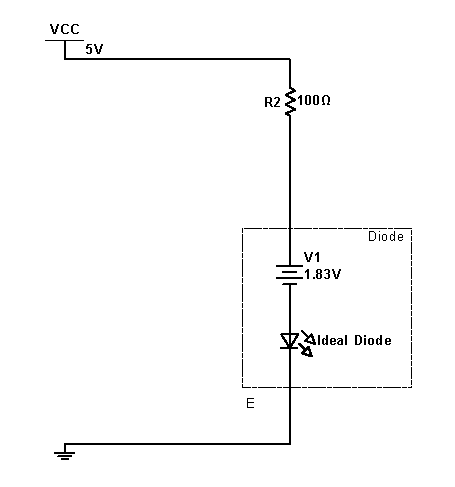
\includegraphics[height=6cm]{LED_control_module_hi_2}

\caption{Equivalent Circuit for High-level}
\end{minipage}
\end{figure}







It is easy to calculate that the current at this time is approximately equal to [\ref{led_control_hi}]:


\begin{equation}
	I_{eq}=\frac{\qty{5}{V} -\qty{1.83}{V}}{\qty{100}{\ohm}}=\qty{31.7}{mA}>\qty{20}{mA} \label{led_control_hi}
\end{equation}


At this time, \verb|LED1| is on and the current is sufficient to illuminate At this time, the corresponding warning light(red LED) is on when the temperature exceeds the set value.


At this time, we analyze the output low level at \verb|C|, and the same $V_C=V_D$, at this time, for \verb|Q1|, $V_{BE} \approx 0 $, BC not conducting.


At this time, \verb|R4| and \verb|R2|, \verb|LED1| are connected in parallel, and the excessive resistance of \verb|R4| can be ignored The circuit diagram is as follows. At this time, since \verb|R7| is a large resistance, the current through \verb|R2| and \verb|LED1| is very small. Therefore, it can obtained that $V_F =0$, so at this time,for \verb|Q1|, $V_{VE} \approx \qty{5}{V} >\qty{0.7}{V}$, \verb}CE} is on, and considering that \verb|LED2| is a green LED with turn on voltage of \qty{2.13}{V}, the circuit diagram can be equivalent to the following:


\begin{figure}[H]
\centering
\begin{minipage}[t]{0.48\textwidth}
\centering
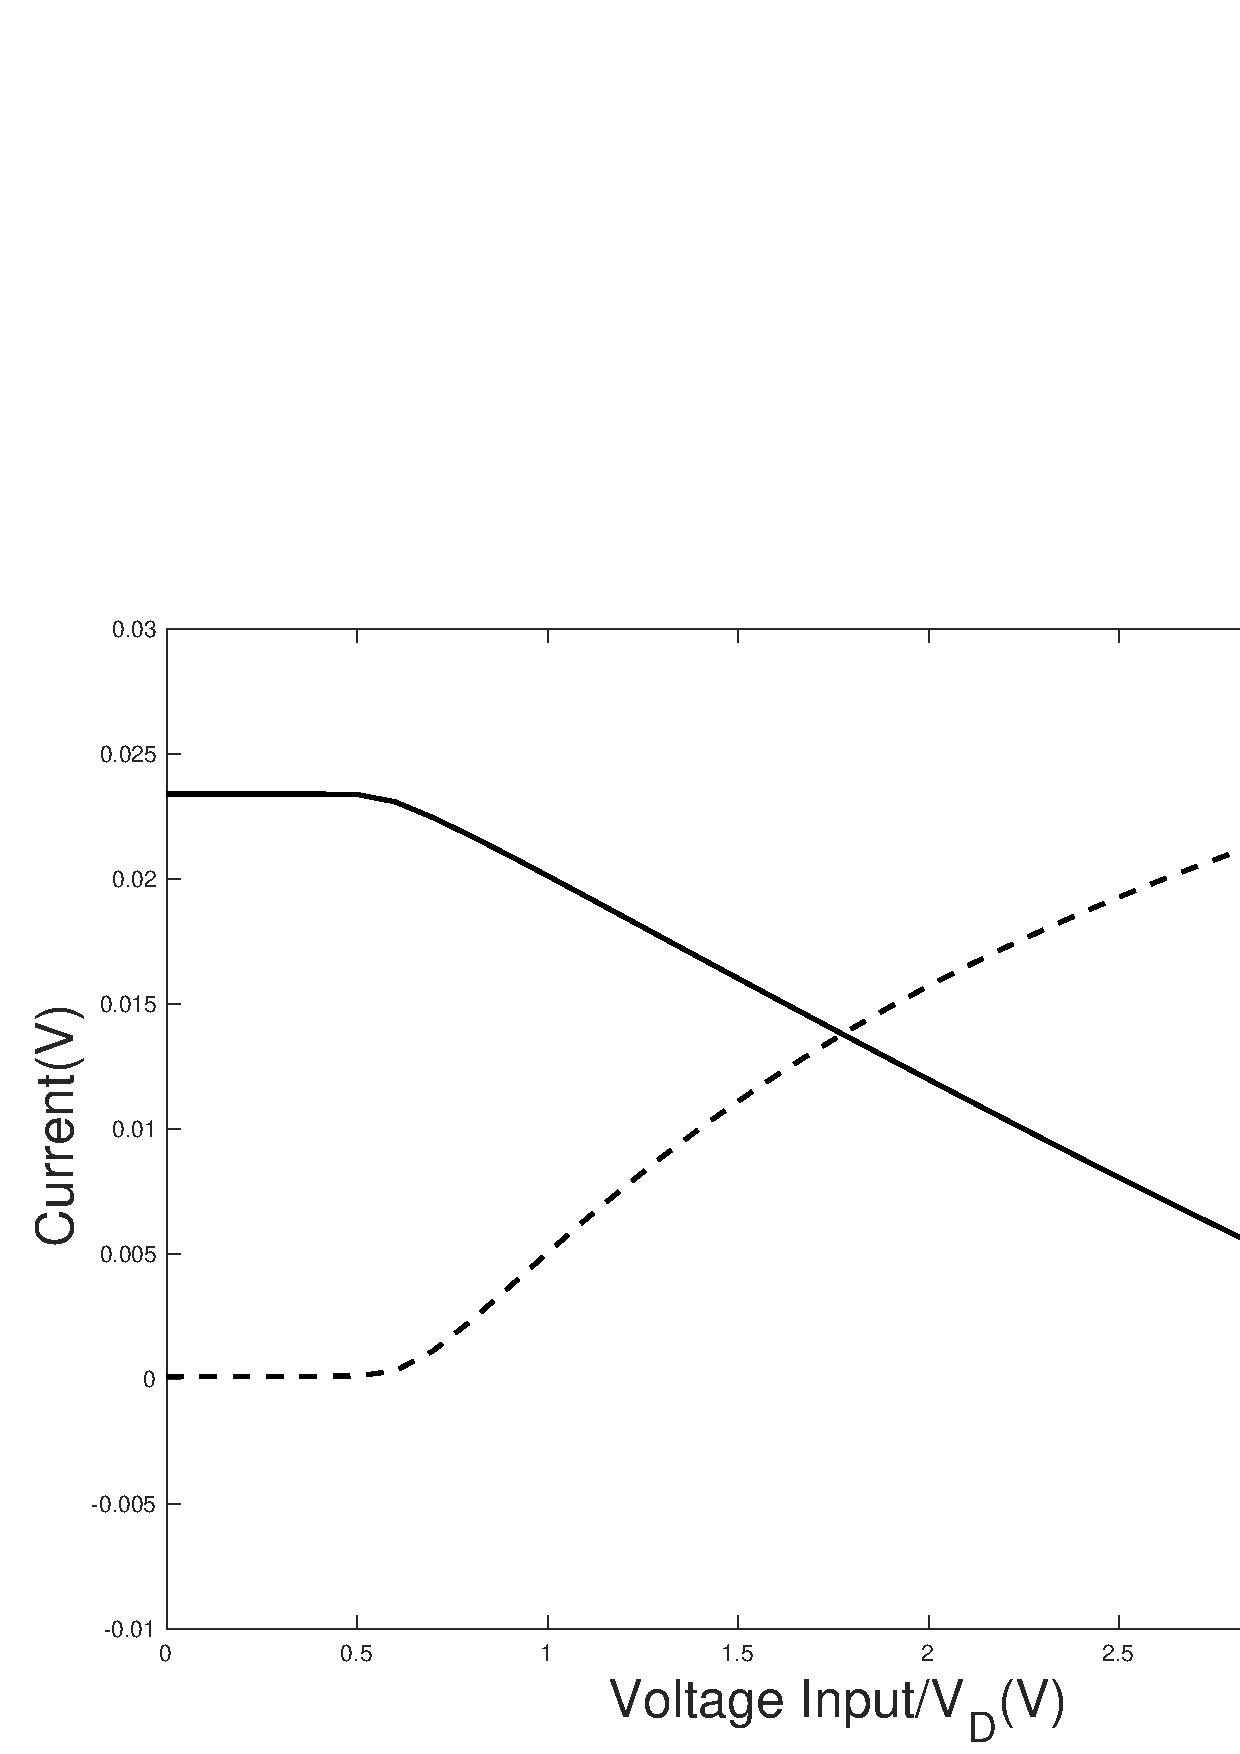
\includegraphics[height=6cm]{LED_control_module_lo_1}

\caption{$V_D=0V$}
\end{minipage}
\begin{minipage}[t]{0.48\textwidth}
\centering
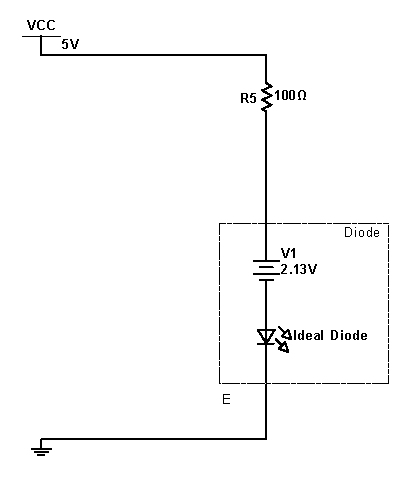
\includegraphics[height=6cm]{LED_control_module_lo_2}
\caption{Equivalent Circuit for Low-level}
\end{minipage}
\end{figure}






Here we can obtain the current flow through \verb|LED2| as [\ref{led_control_lo}]:
\begin{equation}
	I_{eq}=\frac{\qty{5}{V} -\qty{2.13}{V}}{\qty{100}{\ohm}}=\qty{28.70}{mA} >\qty{20}{mA} \label{led_control_lo}
\end{equation}


At this time, \verb|LED2| is on and the current is sufficient to illuminate At this time, the corresponding green light(\verb|LED2|) turns on when the temperature does not exceed the set value
We can add a regulated voltage to the module %TODO 这里加那个有电压的版本
, perform \verb|DC sweep| on it, adjust the voltage from \qtyrange{0}{3.5}{V}, set the increment to \num{0.1}, and perform simulation to output the current through \verb|R2| and \verb|R5|, that is, the current through \verb|LED1| and \verb|LED2|, so as to reflect the circuit conduction state. The image is as follows:


\begin{figure}[H] %H为当前位置,!htb为忽略美学标准,htbp为浮动图形
\centering %图片居中
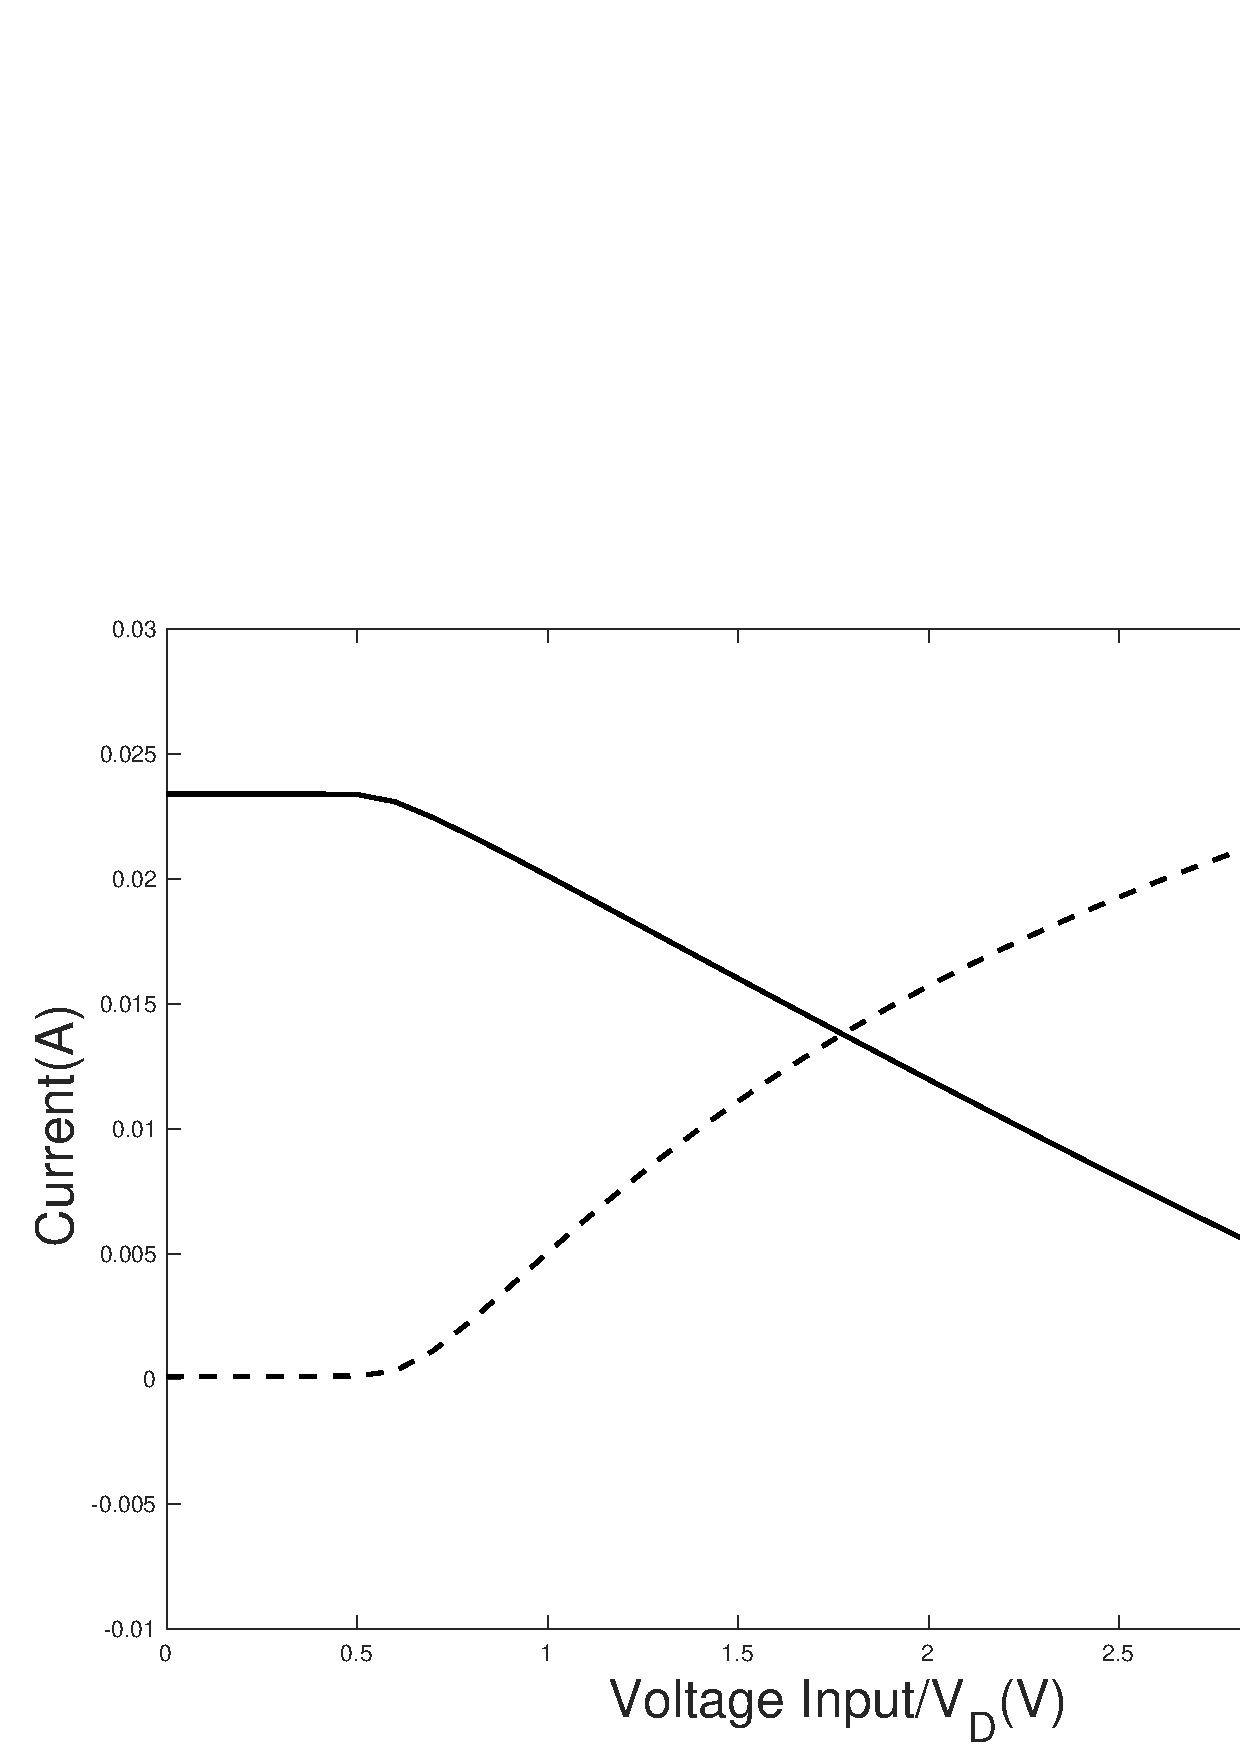
\includegraphics[width=0.8\textwidth]{LED_module_diagram} %插入图片,[]中设置图片大小,{}中是图片文件名
\caption{$I_{RED}$ and $I_{GREEN}$} %最终文档中希望显示的图片标题
\label{Fig.LED_module_diagram} %用于文内引用的标签
\end{figure}


Result is as the same as we expected in analysis.



\subsubsection{Total Simulation}

We combine the two modules, connect the \verb|VOUT| port of Op-Amp with the switch port of LED control module, and connect them to the voltage of \qty{5}{V}. At this time, we need to use the state when the sliding rheostat is set at $40\%$ as an example. At this time, through the previous description, at this time, $V_{OUT}=\qty{0}{V}$ below \qty{60}{\degreeCelsius}. At this time, in the LED control module, \verb|LED2| is on. When the temperature exceeds \qty{60}{\degreeCelsius}, \verb|VOUT| outputs a high level of \qty{3.5}{V}, and \verb|LED2| in the LED control module is turned on, we use \verb|Multisim| for \verb|Temperature Sweep| analysis to linearly increase the temperature from \qtyrange{2}{100}{\degreeCelsius}, and the sampling points are still \num{100}, so that it outputs $I_{R2}$ and $I_{R_5}$ is used to reflect the on state of the circuit.Result below

% TODO 插入图片 total_sweep


\begin{figure}[H] %H为当前位置,!htb为忽略美学标准,htbp为浮动图形
\centering %图片居中
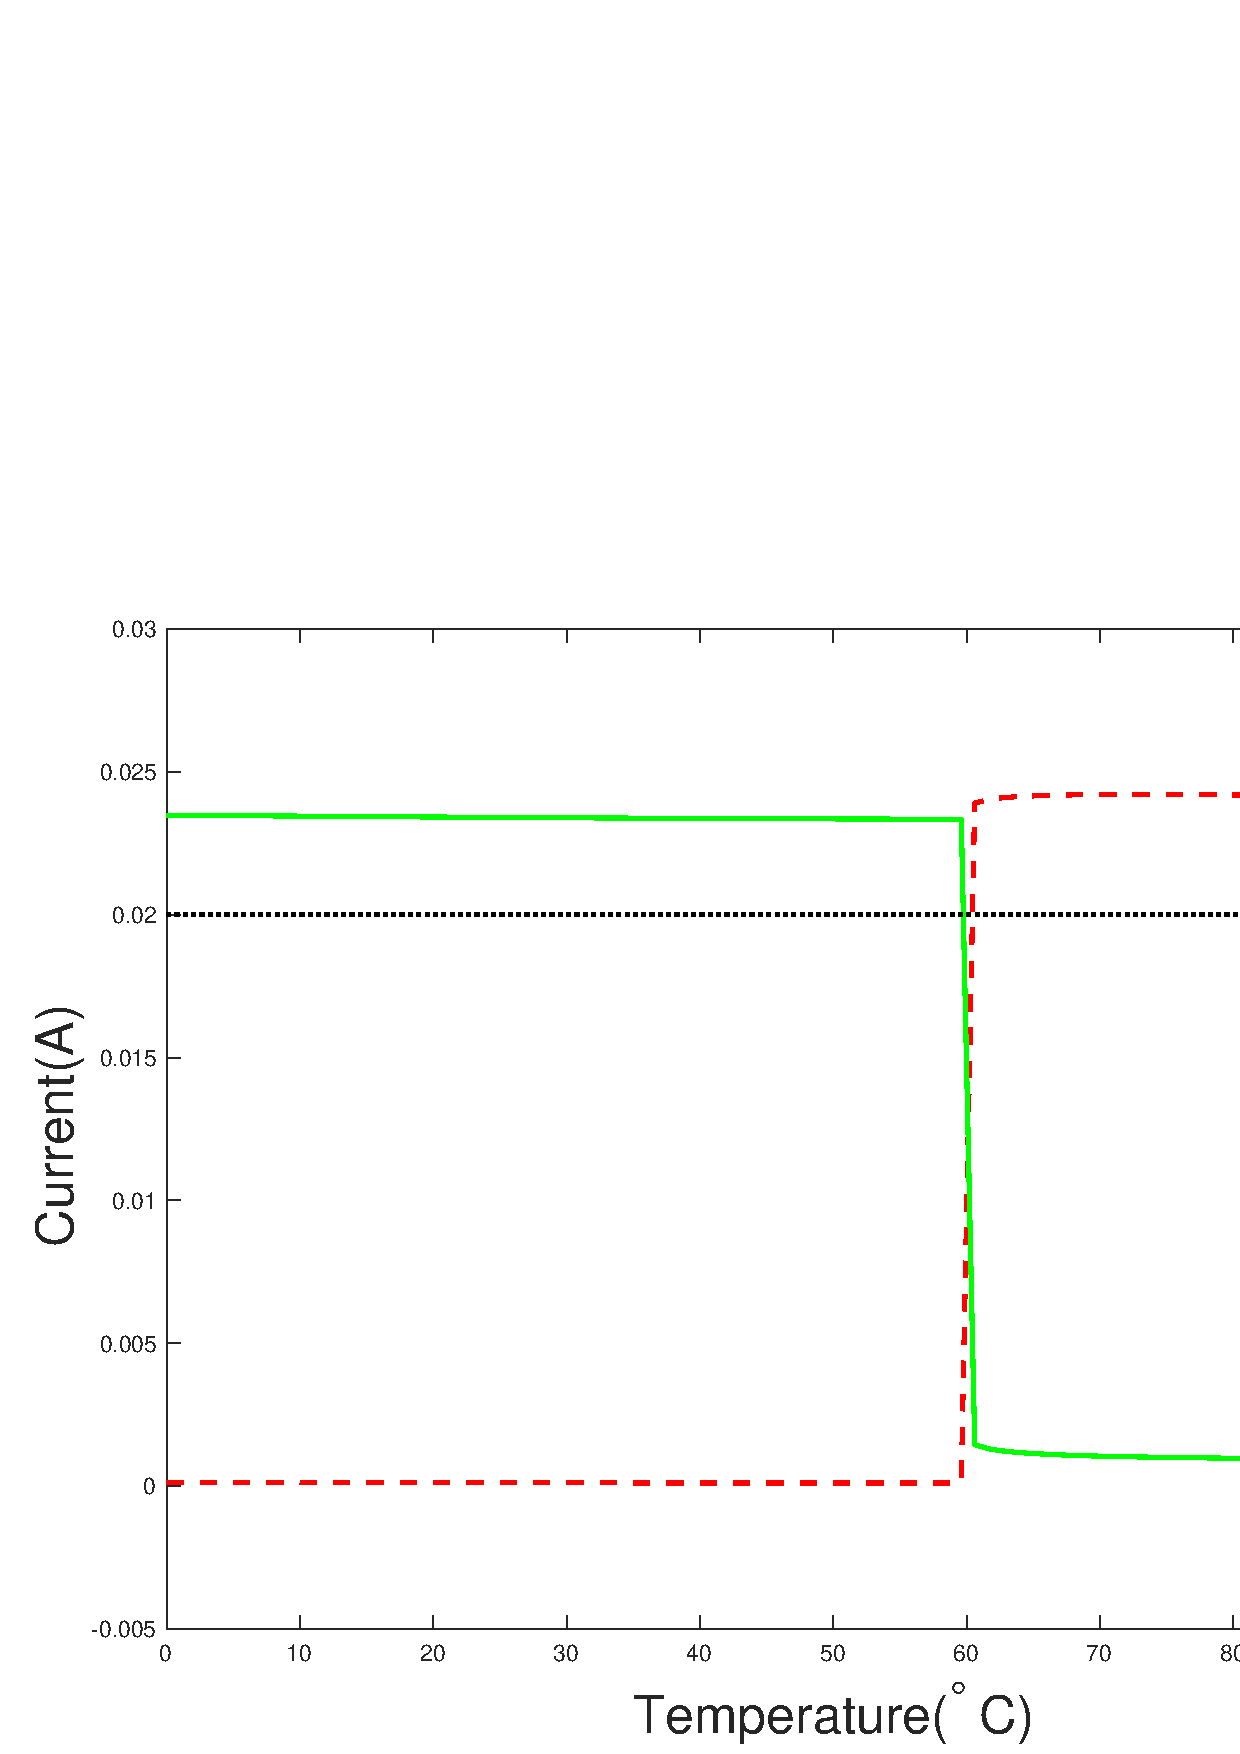
\includegraphics[width=0.8\textwidth]{total_sweep} %插入图片,[]中设置图片大小,{}中是图片文件名
\caption{$I_{RED}$ and $I_{GREEN}$ when temperature sweep} %最终文档中希望显示的图片标题
\label{Fig.temperature_sweep_diagram} %用于文内引用的标签
\end{figure}


It can be seen from our analysis that the green light is always on when the temperature is less than \qty{60}{\degreeCelsius}. When the temperature is close to \qty{60}{\degreeCelsius}, the two temperatures quickly jump off to the other state. When the temperature exceeds  \qty{60}{\degreeCelsius}, the red light is on.


\section{Furthermore}


Through this circuit, people can easily set the temperature and monitor the circuit, which greatly facilitates and improves the quality of life and safety.


At the same time, we can make basic adjustments to the circuit to make it more in line with the needs of life:


\subsection{Battery as power scheme}
The operating voltage of the circuit is \qty{5}{V}, but in life, the voltage of the dry battery is often \qty{1.5}{V}. Therefore, we can convert the \qty{6}{V} voltage of the four dry batteries into a stable \qty{5}{V} voltage by adding a voltage stabilizing diode or a voltage stabilizing LDO in the circuit, and then input the circuit to facilitate people's use The following figure shows the voltage stabilizing circuit made by zener-diode [\ref{Fig.zener}] and its output stable voltage, which is stable at about \qty{5.00}{V}.


\begin{figure}[H] %H为当前位置,!htb为忽略美学标准,htbp为浮动图形
\centering %图片居中
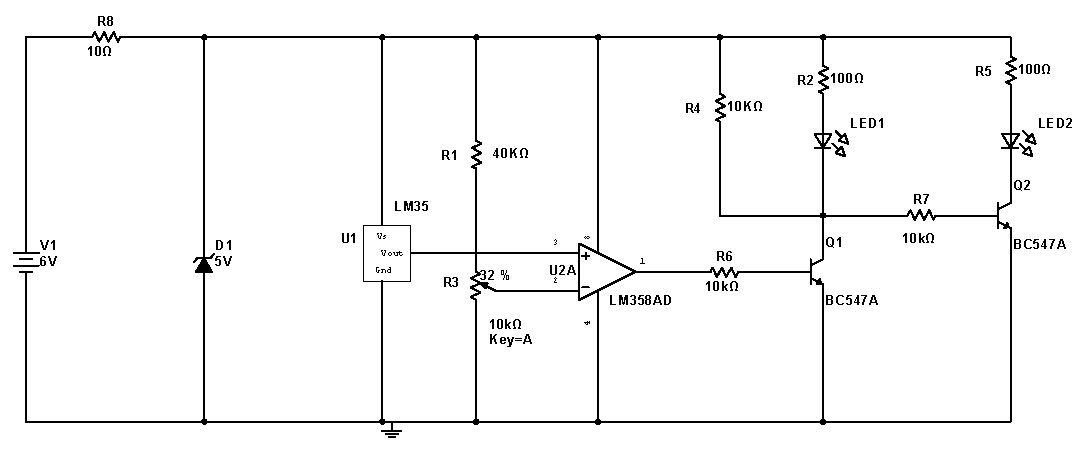
\includegraphics[width=1\textwidth]{zener} %插入图片,[]中设置图片大小,{}中是图片文件名
\caption{Voltage Reduction with 5V-Zener-diode} %最终文档中希望显示的图片标题
\label{Fig.zener} %用于文内引用的标签
\end{figure}



The zener diode is not very suitable. It can be seen from the figure that the resistance connecting the zener diode will produce additional power consumption. %TODO 插入ref

\begin{figure}[H] %H为当前位置,!htb为忽略美学标准,htbp为浮动图形
\centering %图片居中
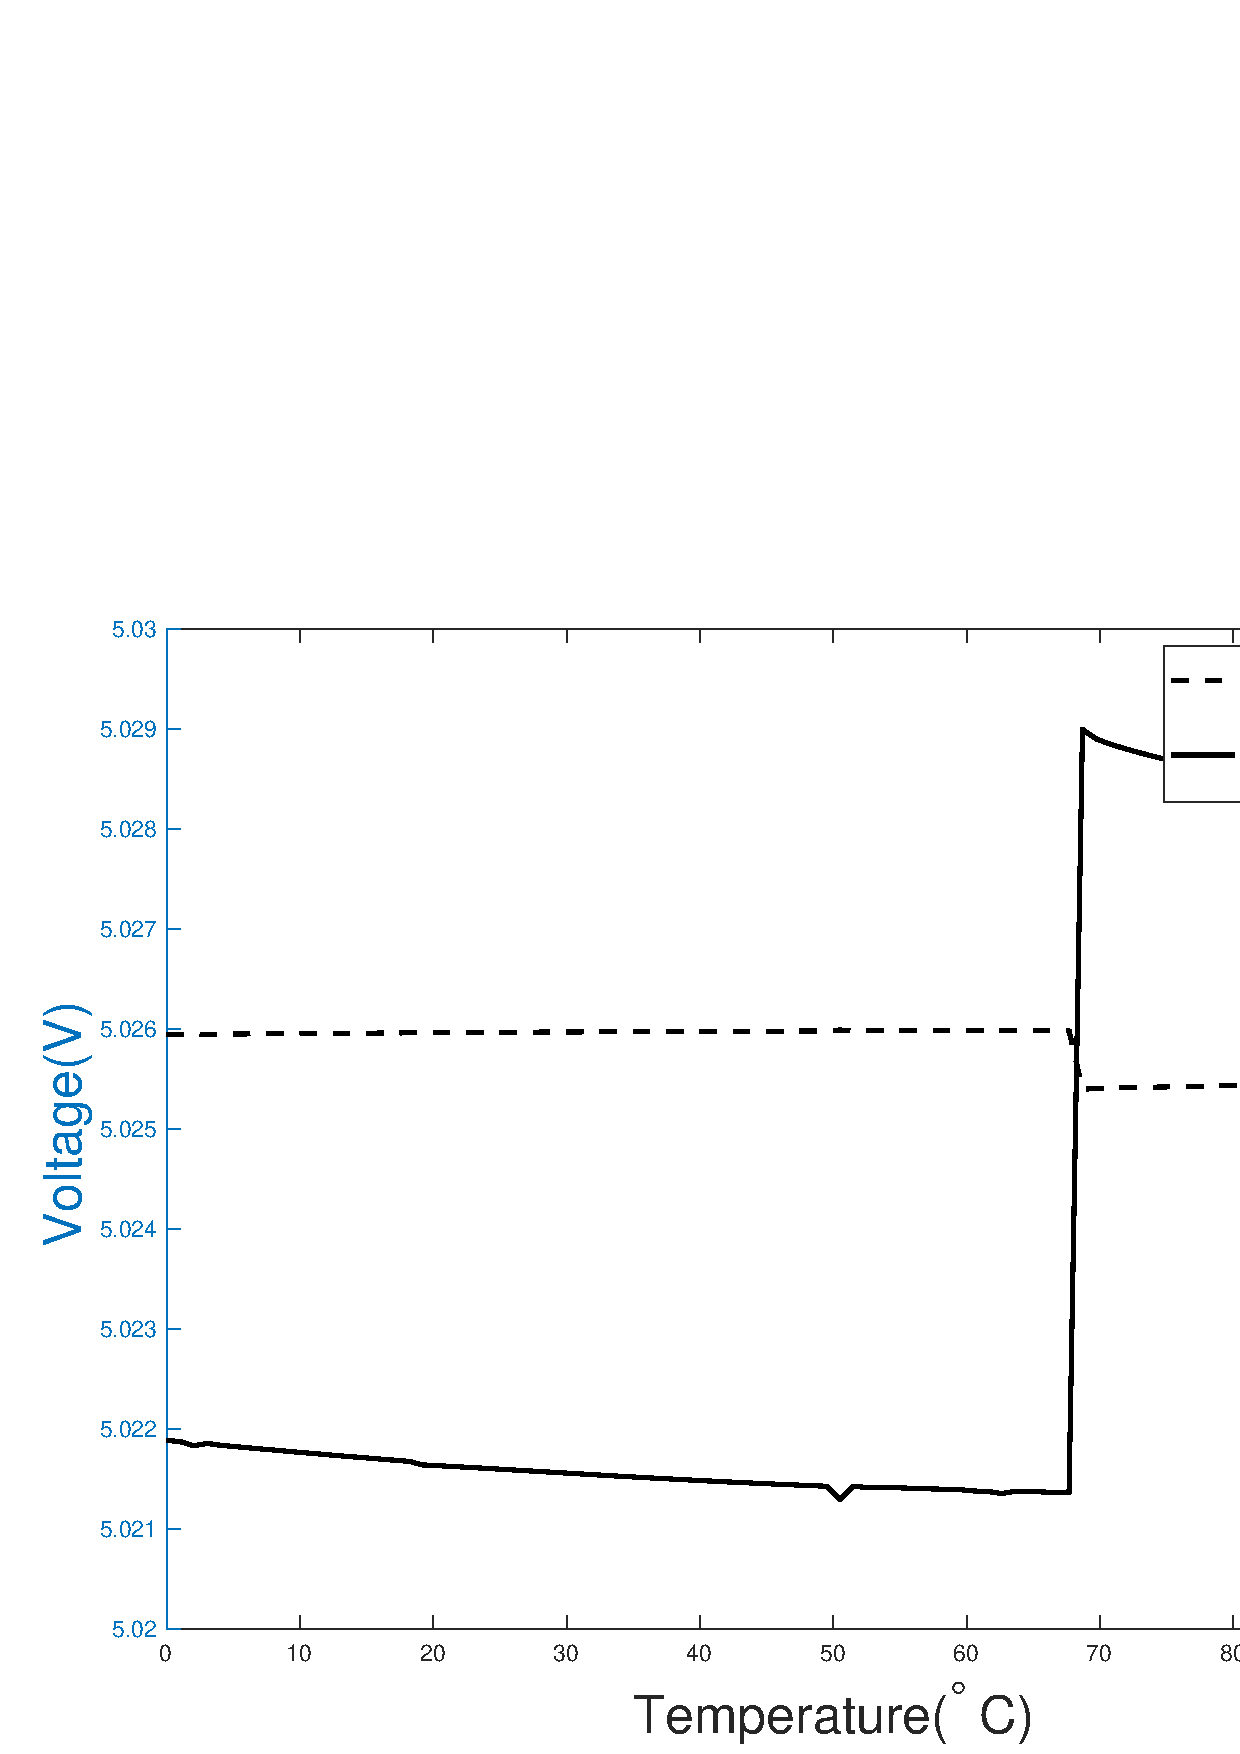
\includegraphics[width=0.7\textwidth]{zener_diagram} %插入图片,[]中设置图片大小,{}中是图片文件名
\caption{Voltage after reduction and Power Loss on R8} %最终文档中希望显示的图片标题
\label{Fig.zener_diagram} %用于文内引用的标签
\end{figure}


\subsection{Add other device for better use}
Some results of temperature switch can be used as switches to control other equipment, such as connecting electrical appliances with temperature regulation function, such as water heater and fan, so as to realize negative feedback regulation of temperature and maintain constant temperature or connect it to the buzzer [\ref{Fig.buzzer}] to indicate a stronger warning.

%TODO 插图 buzzer_module

\begin{figure}[H] %H为当前位置,!htb为忽略美学标准,htbp为浮动图形
\centering %图片居中
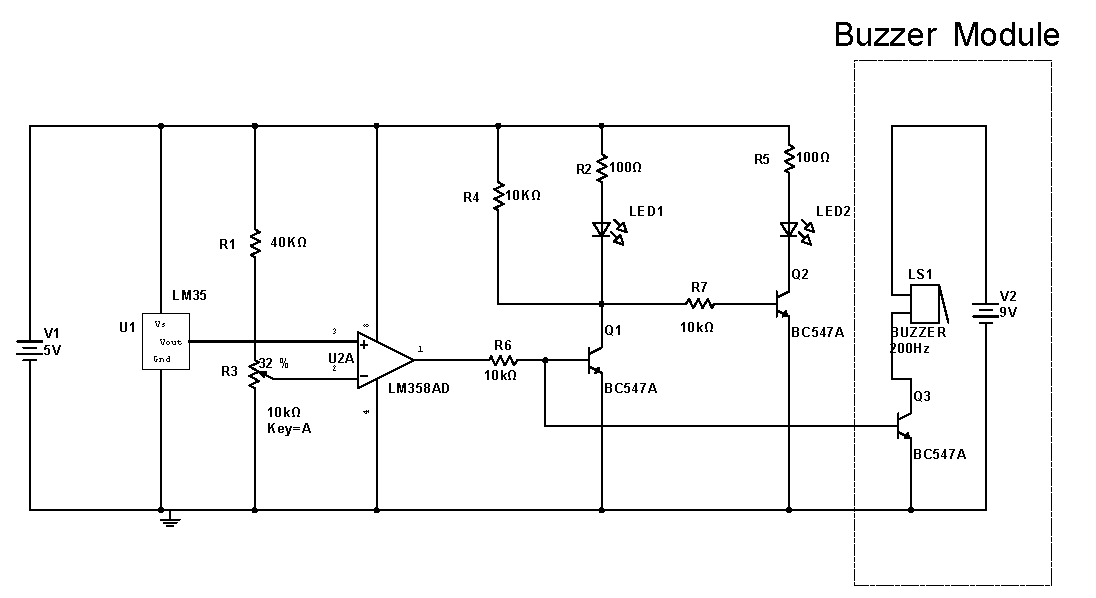
\includegraphics[width=0.7\textwidth]{buzzer_module} %插入图片,[]中设置图片大小,{}中是图片文件名
\caption{Add Buzzer module} %最终文档中希望显示的图片标题
\label{Fig.buzzer} %用于文内引用的标签
\end{figure}


\subsection{For low-emperature use}
In some application scenarios, the operating temperature may be lower, but because the connection mode of \verb|LM35| sensor in the circuit is Basic Contigrade Temperature Sensor [\ref{Fig.basic_contigrade}], we can realize the full range measurement of \verb|LM35| by adjusting the wiring mode to monitor the environment below \qty{0}{\degreeCelsius} [\ref{Fig.low}].

\begin{figure}[H] %H为当前位置,!htb为忽略美学标准,htbp为浮动图形
\centering %图片居中
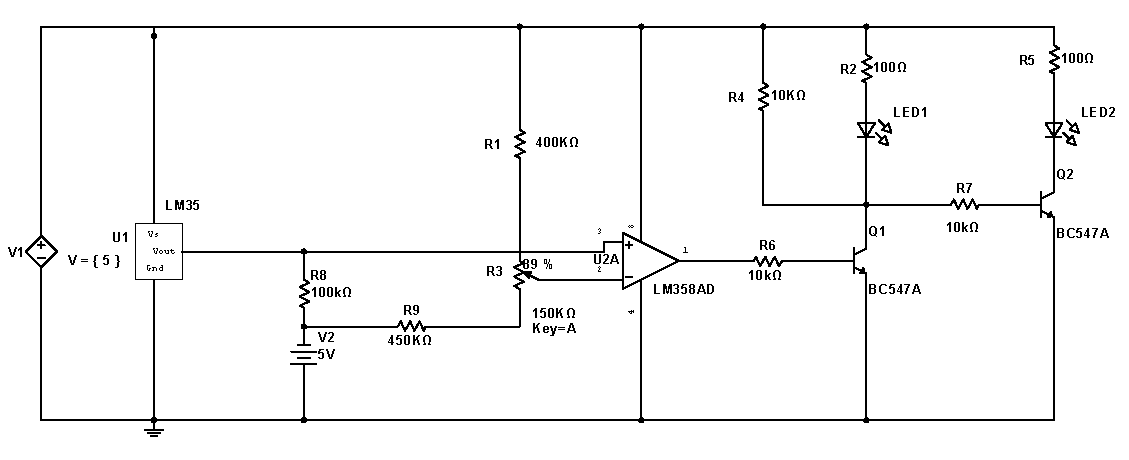
\includegraphics[width=0.7\textwidth]{low_temp} %插入图片,[]中设置图片大小,{}中是图片文件名
\caption{Full-Range Version Temperature Controlled LED Circuit} %最终文档中希望显示的图片标题
\label{Fig.low} %用于文内引用的标签
\end{figure}



.The potentiometer can be adjusted to adjust the threshold temperature from \qtyrange{50}{100}{\degreeCelsius}, and the relationship [\ref{Fig.low_diagram}] between the corresponding value and percentage is


\begin{equation}
	T_{\text{thresold}}=(-50+150(1-p))\unit{\degreeCelsius}
\end{equation}


\begin{figure}[H] %H为当前位置,!htb为忽略美学标准,htbp为浮动图形
\centering %图片居中
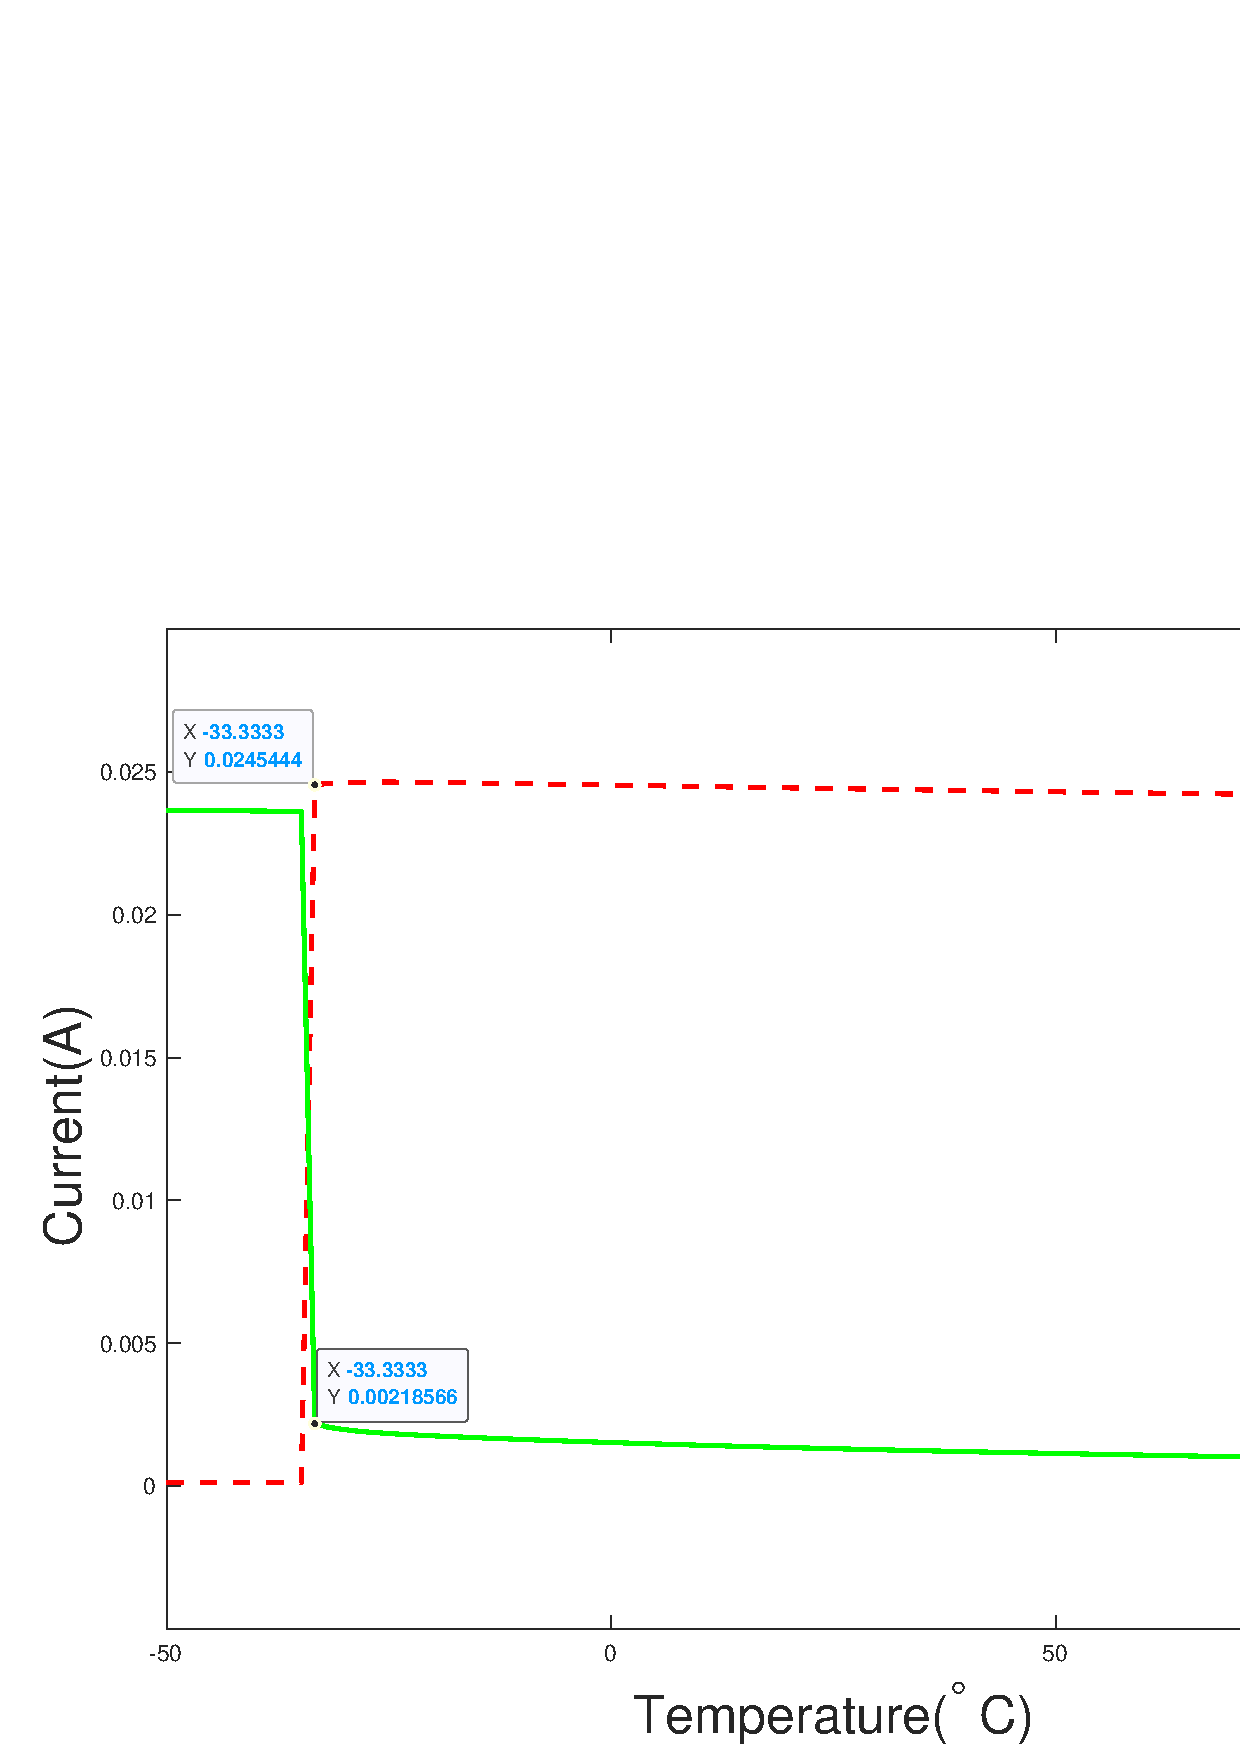
\includegraphics[width=0.7\textwidth]{low_diagram} %插入图片,[]中设置图片大小,{}中是图片文件名
\caption{Thresold Temperature below $0 ^\circ C$ in Full range measurement} %最终文档中希望显示的图片标题
\label{Fig.low_diagram} %用于文内引用的标签
\end{figure}
%TODO 插图 low_diagram





\subsection{Range-monitoring System}
In daily life, we often need a fixed temperature range rather than a single temperature threshold. Therefore, we can design the following two circuits: 2-light temperature control range LED and 3-light temperature control range LED.People can set the upper and lower temperature limits by adjusting two potentiometers.
\begin{enumerate}
	\item In the 2 light version [\ref{Fig.2light}], as long as the temperature exceeds the temperature range corresponding to the potentiometers, the red light(\verb|LED1|) will be turned on and the green light(\verb|LED2|) will be turned off.
	\item In the 3 light version [\ref{Fig.3light}], when the temperature is higher than the set maximum temperature, the high temperature warning light (red \verb|LED2|) will light up, and when the temperature is lower than the set minimum temperature, the low temperature warning light (blue \verb|LED1|) will light up.
	\item When the temperature is within the set range, the green light(\verb|LED3|) are on.
\end{enumerate}

Here set the \verb|Tmin|(\verb|R8|) and \verb|Tmax|(\verb|R3|),then we can obtaint the diagram of the current flow through the LED lights with 2 light version and 3 light version,respectively.


\begin{figure}[H] %H为当前位置,!htb为忽略美学标准,htbp为浮动图形
\centering %图片居中
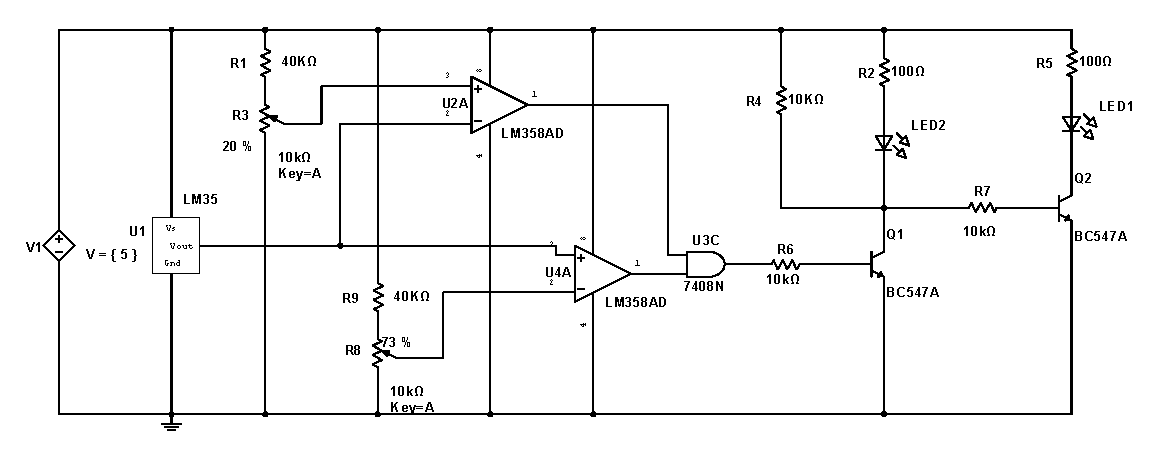
\includegraphics[width=\textwidth]{2light_range} %插入图片,[]中设置图片大小,{}中是图片文件名
\caption{2-light temperature control range LED} %最终文档中希望显示的图片标题
\label{Fig.2light} %用于文内引用的标签
\end{figure}



% 2led_range_diagram

\begin{figure}[H] %H为当前位置,!htb为忽略美学标准,htbp为浮动图形
\centering %图片居中
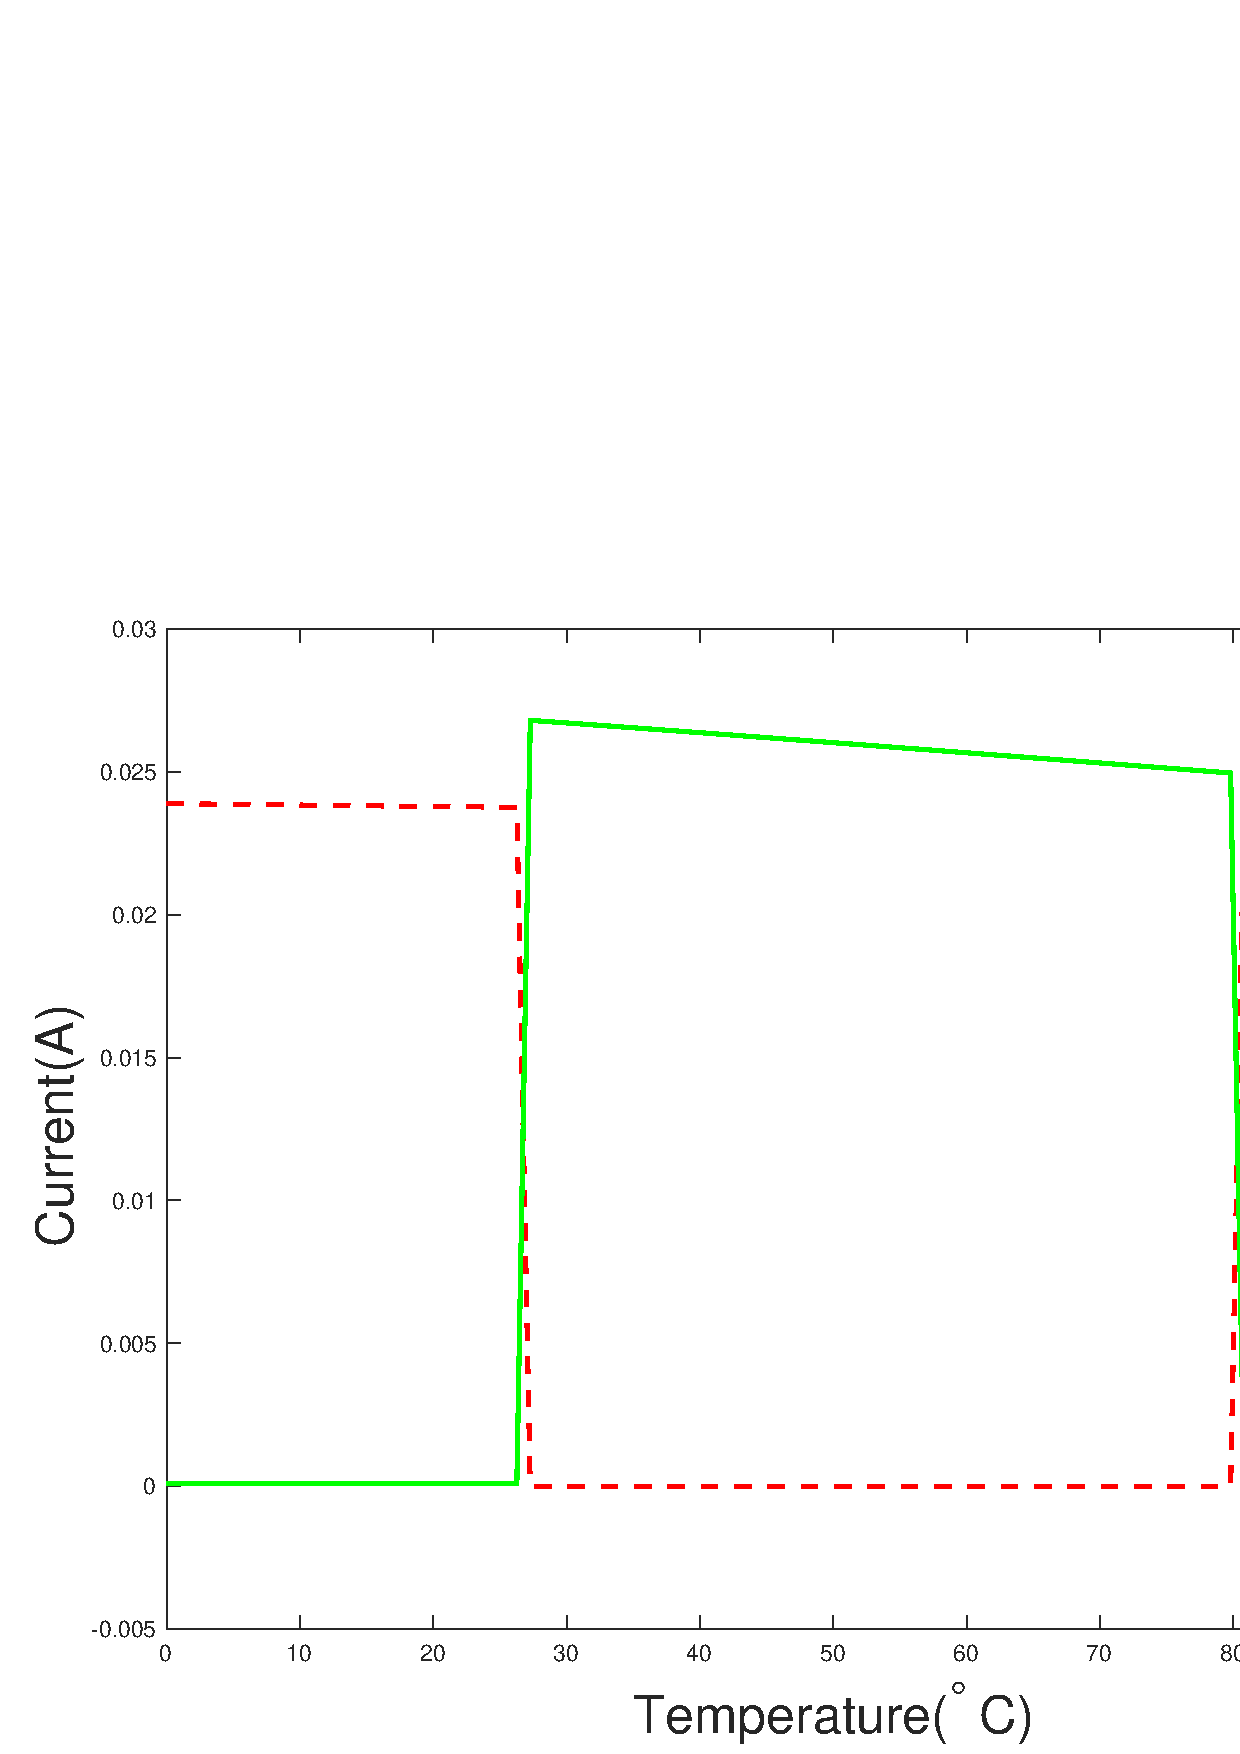
\includegraphics[width=\textwidth]{2led_range_diagram} %插入图片,[]中设置图片大小,{}中是图片文件名
\caption{Current pass LED in 2-light temperature control range LED} %最终文档中希望显示的图片标题
\label{Fig.2light_diagram} %用于文内引用的标签
\end{figure}





\begin{figure}[H] %H为当前位置,!htb为忽略美学标准,htbp为浮动图形
\centering %图片居中
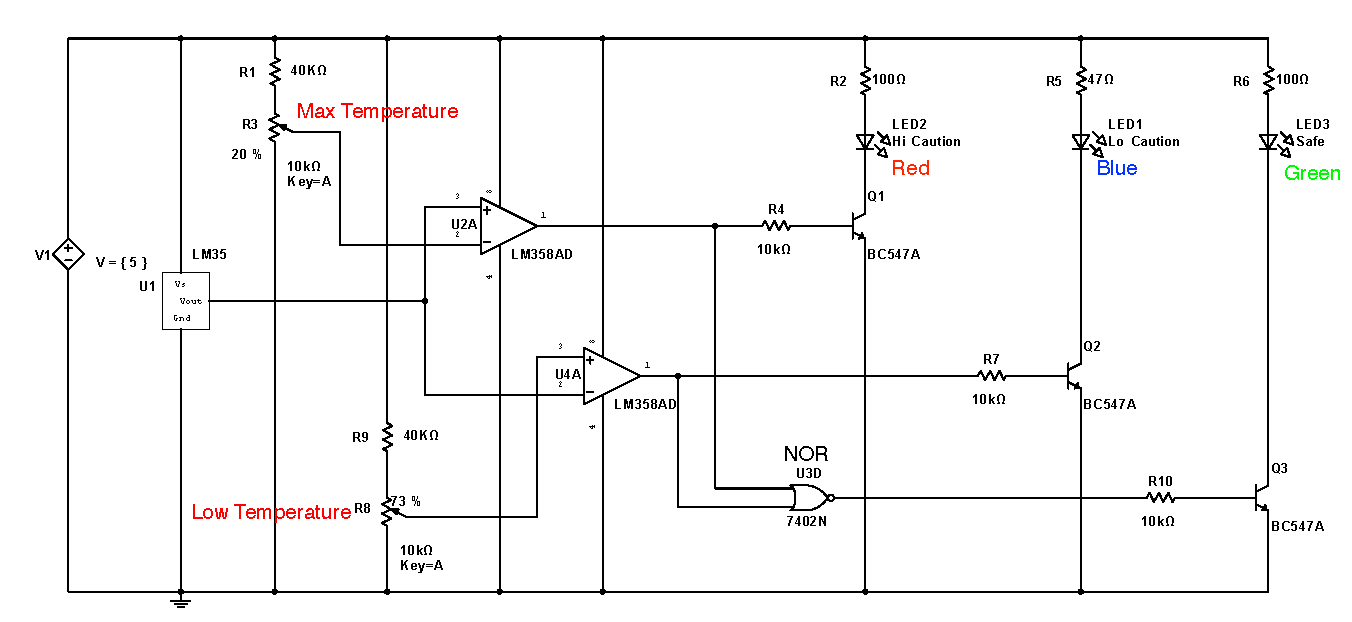
\includegraphics[width=\textwidth]{3light_range} %插入图片,[]中设置图片大小,{}中是图片文件名
\caption{3-light temperature control range LED} %最终文档中希望显示的图片标题
\label{Fig.3light} %用于文内引用的标签
\end{figure}

\begin{figure}[H] %H为当前位置,!htb为忽略美学标准,htbp为浮动图形
\centering %图片居中
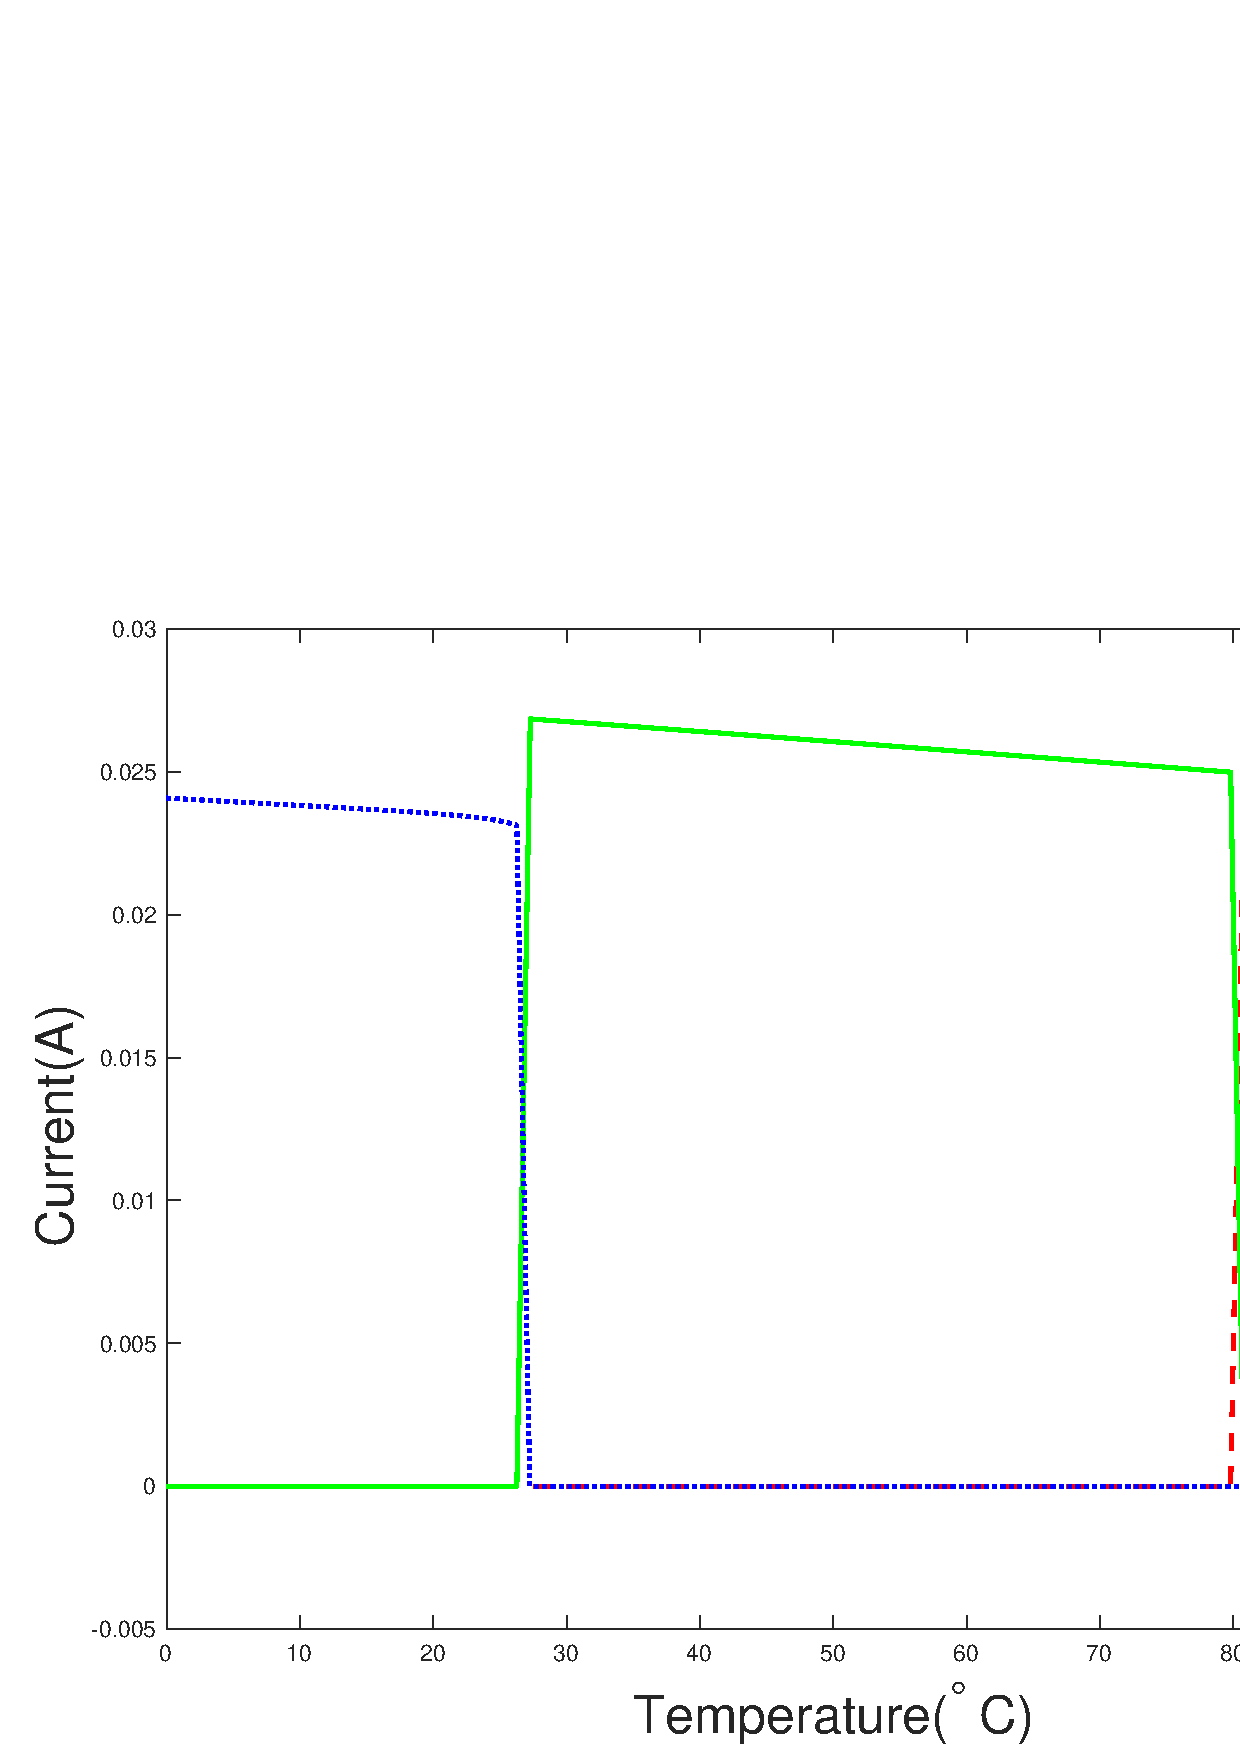
\includegraphics[width=\textwidth]{3_range_diagram} %插入图片,[]中设置图片大小,{}中是图片文件名
\caption{Current pass LED in 3-light temperature control range LED} %最终文档中希望显示的图片标题
\label{Fig.3light_diagram} %用于文内引用的标签
\end{figure}




\newpage
\bibliographystyle{IEEEtran}
\bibliography{ref}


\appendix

\section{Attached File}
The output data, diagram, Multisim file, plot program attached in Github(\href{https://git.io/JyctL}{https://git.io/JyctL}).  



\section{Full Diagram}















\end{document}